\subsection{平稳分布与特殊例子}

\[
(X_n)_{n\geq 0}\sim \text{Markov}(\mu^{(0)},P)
\]
初始分布 $\mu^{(0)}=(\mu_i^{(0)})_{i\in S}$, 其中 $\mu_i^{(0)}=\PP(X_0=i)$

在 $n$ 时刻的分布, $\mu^{(n)}=(\mu_i^{(n)})_{i\in S}$, 其中 $\mu_i^{(n)}=\PP(X_n=i)$
\[
\mu^{(n)}=\mu^{(0)}P^n
\]
\begin{definition}[平稳分布]
    称概率分布 $\pi=(\pi_i)_{i\in S}$ 是转移矩阵 $P$ 的平稳分布, 若
    \begin{equation}
        \pi P=\pi
        \label{eq:stationary}
    \end{equation}
    注:$\mu^{(n+1)}=\pi P^{n+1}=\pi P\cdot P^n=\pi P^n=\pi P=\pi=\mu^{(0)}$
\end{definition}

\begin{problem}[作业6-4]
    设 $(X_n)\sim \text{Markov}(\pi,P)$, $\pi$是$P$的平稳分布, 证明:对固定 $m\geq 0$, 有 $(X_{m+n})_{n\geq 0}\sim \text{Markov}(\pi,P)$
\end{problem}

\subsubsection{双随机链(Doubly Stochastic Chain)}

回顾随机矩阵定义\ref{thm:random_matrix}, 现在由行和为1, 拓展到列和也为1.

\begin{definition}
    称转移矩阵 $(p_{xy})_{x,y\in S}$ 是双随机的, 若 $\sum_{x\in S}p_{xy}=1$
\end{definition}

\begin{theorem}
    设 $P=(p_{xy})_{x,y\in S}$ 为具有 $N<\infty$ 个状态的马氏链的转移概率矩阵, 且有均匀分布 $\pi_x=\frac{1}{N},x\in S$ 则下面两个命题等价:
\begin{enumerate}
\item $\pi_x$ 是 $P$ 的平稳分布
\item $P$ 双随机
\end{enumerate} 
\end{theorem}

\begin{proof}
$\forall y\in S,\pi_y=\frac{1}{N}$
\[
(\pi P)_y=\sum_{x\in S}\pi_x p_{xy}=\frac{1}{N}\sum_{x\in S}p_{xy}
\]
\begin{enumerate}
    \item $P$双随机, $(\pi P)_y=1/N=\pi_y,(\forall y\in S)\Rightarrow \pi P=\pi$
    \item $(\pi P)_y=\pi_y,\forall y\in S,\frac{1}{N}\sum_{x\in S}p_{xy}=1/N \Rightarrow \sum_{x\in S}p_{xy}=1\Rightarrow P$双随机
\end{enumerate}
\end{proof}

\subsubsection{细致平衡条件(Detailed Balance Condition)}

\begin{definition}
    称概率分布 $\pi$ 满足DBC, 若
    \begin{equation}
        \pi_xp_{xy}=\pi_y p_{yx}\quad (\forall x,y\in S)
    \label{eq:dbc}
    \end{equation}
\end{definition}

注:DBC 是 $\pi P=\pi$ 的充分不必要条件.
\begin{proof}
$\pi P=\pi\iff (\pi P)_y=\pi_y,\forall y\iff\sum_{x\in S}\pi_x p_{xy}=\pi_y,\forall y$. 由于 $\pi_y=\pi_y(\sum_{x\in S} p_{yx})=\sum_{x\in S}\pi_y p_{yx}$,
\begin{equation}
    \pi P=\pi\iff\sum_{x\in S}\pi_x p_{xy}=\sum_{x\in S}\pi_y p_{yx}
    \label{eq:sum_dbc}
\end{equation}
由 $\eqref{eq:dbc}$ 可以推出 $\eqref{eq:sum_dbc}$ 右边等式, 但反之不然.
\end{proof}

\begin{example}[DBC反例]
    $S=\{1,2,3\},N=3$
    \[
    P=\begin{bmatrix}
        0.5 & 0.5 & 0\\
        0.3 & 0.1 & 0.6\\
        0.2 & 0.4 & 0.4
    \end{bmatrix}
    \]
    $P$ 双随机, $\pi=(1/3,1/3,1/3)$ 是 $P$ 的平稳分布
    \begin{claim}
        $\pi$ 不满足 DBC
    \end{claim}
    反证:$\pi$满足DBC$\Rightarrow$ $\pi_x p_{xy}=\pi_y p_{yx}$ 与 $p_{12}=0.5\neq p_{21}=0.3$矛盾\qed
\end{example}

\begin{example}[生灭链]\label{exa:birth_death}
    状态空间 $S=\{l,l+1,\cdots,r-1,r\}\st N_0$, 设 $P$ 满足
    \begin{enumerate}
        \item 一步转移不超过1, 当$|x-y|\geq 2$时, $p_{xy}=0$
        \item $p_{x,x+1}=p_x(\forall x<r)$
        \item $p_{x,x-1}=q_x(\forall x>l)$
        \item $p_{x,x}=1-p_x-q_x(\forall x\in S)$
    \end{enumerate}
    求出 $P$ 的满足DBC条件的平稳分布$\pi$, rf.\eqref{eq:dbc}.
\end{example}

\begin{enumerate}
    \item $|x-y|\geq 2$时, $p_{xy}=p_{yx}=0$
    \item $x=y$时, $p_{xy}=p_{yx},\pi_x=\pi_y$
    \item $y=x+1$时, $(x<r),\pi_x p_{x,x+1}=\pi_{x+1}p_{x+1,x}$
\end{enumerate}
\[
\pi_{x+1}=\frac{\pi_x p_{x,x+1}}{p_{x+1,x}}=\pi_x\frac{p_x}{q_{x+1}}
\]
\[
\pi_{l+n}=\overbrace{\underbrace{\pi_l\frac{p_l}{q_{l+1}}}_{\pi_{l+1}} \frac{p_{l+1}}{q_{l+2}}}^{\pi_{l+2}}\cdots \frac{p_{l+n-1}}{q_{l+n}}
\]
令 
\[a_0=1,a_1=\frac{p_l}{q_{l+1}},a_2=\frac{p_l p_{l+1}}{q_{l+1} q_{l+2}},\cdots,a_{r-l}=\frac{p_lp_{l+1}\cdots p_{r-1}}{q_{l+1}q_{l+2}\cdots q_r}
\]
则 $\pi=(\pi_l a_0,\pi_l a_1,\cdots, \pi_l a_{r-l})$. 又 $\sum_{x\in S}\pi_x=1$, 则
\[
\pi_l\sum_{0\leq n\leq r-l}a_n=1\Rightarrow \pi_l=\frac{1}{\sum_{0\leq n\leq r-l}a_n}
\]
记 $a:=\sum_{0\leq n\leq r-l}a_n$, 则 $\pi=(a_0/a,a_1/a,\cdots,a_{r-l}/a)$\qed

\subsubsection{可逆性}

\begin{theorem}
    设 $(X_n)_{n\geq 0}\sim \text{Markov}(\pi,P)$, 其中 $\pi$ 是 $P$ 的平稳分布.固定$n$, 令 $Y_m:=X_{n-m}(0\leq m\leq n)$, 则
    \[
    (Y_m)_{0\leq m\leq n}\sim\text{Markov}(\pi,\hat{P})
    \]
    其中 $\hat{P}=(\hat{p}_{ij})_{i,j\in S}$
    \[
    \hat{p}_{ij}=\frac{\pi_j p_{ji}}{\pi_i}
    \]
    这里 $\hat{p}_{ij}$ 称为对偶(dual)转移概率
\end{theorem}
\begin{proof}
先验证 $(Y_m)_{0\leq m\leq n}\sim \text{Markov}(\pi,\hat{P})$, 用定义/有限维分布. 这里用定义验证.

(Step 1) 验证 $\hat{P}$ 是随机矩阵
\begin{enumerate}
    \item 元素非负 $\hat{p}_{ij}\geq 0$
    \item $\sum_{j\in S}\hat{p}_{ij}=\sum_{j\in S}(\pi_j p_{ji}/\pi_i)=\pi_i/\pi_i=1$, rf.\eqref{eq:stationary}
\end{enumerate}

(Step 2) 验证初始分布.由 \eqref{eq:stationary} , 初始分布 $Y_0=X_n\sim \pi$

(Step 3) 验证马氏性
\[
\begin{aligned}
    \PP(Y_{m+1}=i_{m+1}|Y_m=i_m,\cdots,Y_1=i_1,Y_0=i_0)&=\frac{\PP(Y_{m+1}=i_{m+1},\cdots,Y_0=i_0)}{\PP(Y_m=i_m,\cdots,Y_0=i_0)}\\
    &=\frac{\PP(X_{n-m-1}=i_{m+1},\cdots,X_{n-1}=i_1,X_n=i_0)}{\PP(X_{n-m}=i_m,\cdots,X_n=i_0)}\\
    &=\frac{\pi_{i_{m+1}}P_{i_{m+1},i_m}\cdots P_{i_1,i_0}}{\pi_{i_m}P_{i_m,i_{m-1}}\cdots P_{i_1,i_0}}\\
    &=\frac{\pi_{i_{m+1}}P_{i_{m+1},i_m}}{\pi_{i_m}}=\hat{p}_{i_m,i_{m+1}}
\end{aligned}
\]
\end{proof}

\begin{corollary}[可逆性]
    若 $P$ 的平稳分布为 $\pi$, 满足 DBC 条件\eqref{eq:dbc}, 则 $\hat{P}=P$.即原来的链$\overset{(d)}{=}$逆向链(记号$\overset{(d)}{=}$表示同分布)
\end{corollary}
\begin{proof}
$\hat{p}_{ij}=(\pi_j p_{ji})/\pi_i\overset{\text{DBC}}{=}(\pi_i p_{ij})/\pi_i=p_{ij}$
\end{proof}

\subsubsection{求$P$的平稳分布(若唯一)}
\[
\begin{cases}
    \pi P=\pi\\
    \sum_{x}\pi_x=1(\pi_x\geq 0,\forall x)
\end{cases}\quad \Rightarrow \quad
\begin{cases}
    \pi(P-\II)=0\\
    \sum_x\pi_x=1
\end{cases}
\]
\begin{example}
例 [Durrett, 1.19]
    \begin{figure}[H]
        \centering
        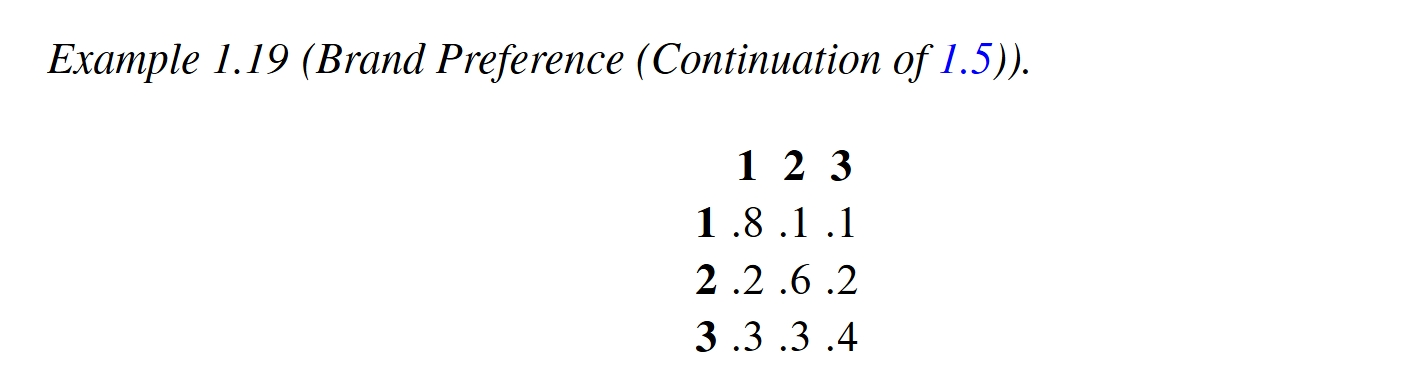
\includegraphics[width=0.9\textwidth]{figures/1_19.png}
    \end{figure}
\end{example}
\[
P-\II=\begin{bmatrix}
    -0.2 & 1 & 1\\
    0.2 & -0.4 & 0.2\\
    0.3 & 0.3 & -0.6
\end{bmatrix}
\]
\[
\begin{cases}
    \pi P=\pi\\
    \sum_{x}\pi_x=1(\pi_x\geq 0,\forall x)
\end{cases}\quad \Rightarrow \quad
\begin{cases}
    -0.2\pi_1+0.2\pi_2+0.3\pi_3=0\\
    \pi_1-0.4\pi_2+0.3\pi_3=0\\
    \pi_1+0.2\pi_2-0.6\pi_3=0\\
    \pi_1+\pi_2+\pi_3=1
\end{cases}
\]
前三个等式是线性相关的, 删去一个等式
\[
A=\begin{bmatrix}
    -0.2 & 1 & 1\\
    0.2 & -0.4 & 1\\
    0.3 & 0.3 & 1
\end{bmatrix},\quad b=[0,0,1]
\]
$\pi A=b\Rightarrow \pi=bA^{-1}$, 即 $A^{-1}$ 的最后一行

\newpage